\section{Sequential Composition of Dynamically Dexterous Robot Behaviors}
Authors: D.E. Koditschek\\
Year: 2015
\subsection*{Summary}
\begin{itemize}
\item Preimage backchaining concept is defined as inspired by [Lozano-Perez,Mason,Taylor 1984].
\item In this paper a clear approach to the problem of hybrid systems is given. An hybrid control problem is here defined as the problem of defining a control for a mix of continuous and discrete systems.
\item The coupled robot-environment state must be considered, not just one.
\item ''Event driven'' trajectory generators are needed.
\item The concept of invariant ellipsoid is given as the ellipsoid in the phase plane where the ball can be safely sent and there it does not lead to failure
\item Basically three different controllers are defined: juggling, catching and palming. Each of them is defined on a different sub-domain and a passage from one to another is made possible just thanks to a higher-level controller which sets the path to the goal.
\begin{figure}
  \centering
  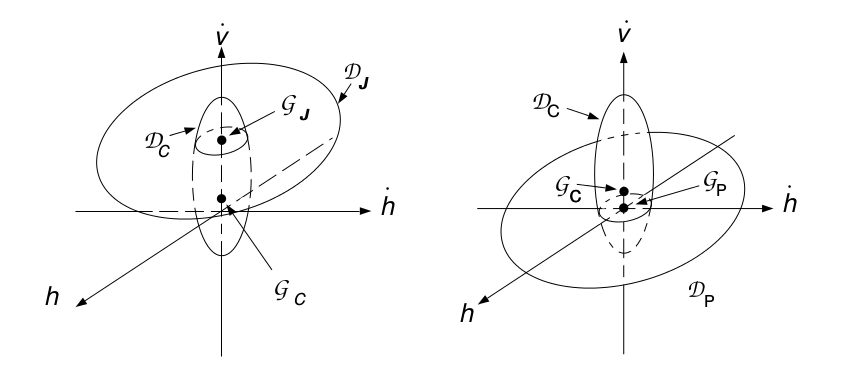
\includegraphics[width=90mm]{Koditschek1}
  \caption{Representation of the three different domains of the three controllers: juggle, catcher and palmer}
  \label{PhasePlane}
\end{figure}
\end{itemize}

\subsection*{Key points / Takeaways}
\begin{enumerate}
\item A \textit{pre-image}, in the paper of Lozano-Perez, can be seen as the set of all the points of the space that allow to reach a goal with a single discrete motion
\item The term \textit{back chaining} refers to process of splitting the trajectory from the goal back to the starting point in many \textit{pre-images} that corrispond to discrete movements.
\item It is shown that the vertical velocity $\dot{z}$ has little influence when compared to the general horizontal speed $\dot{h}$ (either $\dot{x}$ or $\dot{y}$).
\end{enumerate}
\subsection*{Weak points}
\subsection*{Ideas}
\begin{enumerate}
\item Extend the idea of \textit{self-manipulation}: what if we reverse the problem of locomotion and we look at it as a manipulation problem? It is like considering that the earth is moving and the robot is a fixed frame. The manipulation consists in this case of many impacts which keep the earth in the "controllable region". 
\item analyse a way to approach the control of \textbf{Discrete Events Systems}. In between two following events the system can thus be seen as an \textbf{autonomous system} (we cannot change the trajectory of the CoM between two events, what we can do is only to adjust the angular orientation and the position of the feet at the next impact).
\item From the manipulation point of view: we deal with the control of a DES when we have an obstacle which disconnects the workspace.
\end{enumerate}
